%-------------------------------------------------------------------------------
%	CAPITOLO 30
%-------------------------------------------------------------------------------

\chapter{Il fanale ed i bisognosi di un albero}
Col suffragio elettorale allargato e l'aumento della popolazione la legge che pretende di regalare tutto dava al paese 30 consiglieri. Cominciarono le spese per preparare i posti per farli sedere e questo fu il primo danno. Il secondo danno fu lo sciupio di carta, sottratta ai WC per la loro elezione... e così via.\\
\indent La passata amministrazione dei monarchici, aveva fatto collocare un fanale a gasolina presso il \index[Luoghi]{Ponte della Ferrovia}Ponte della Ferrovia per rischiarare il passaggio a livello, l'argine del fiume e la rampa che va al \index[Luoghi]{Borgo Gallina}Borgo Gallina.\\
\indent In una seduta si alza il consigliere S.\: \: del \index[Luoghi]{Borgo Gallina}Borgo Gallina, chiamata ed ottenuta la parola, dice: <<A feg la pruposta d'cavè e lampiòn d'in se pont d'la feroveia, parchè su iè un quelcadun ch'eva bsogn d'andes a tu un élbar in te cant \index[Personaggi]{Alberani Anselmo}d'Albarèn, cui possa andè senza èsar vèst\footnote{<<Faccio la proposta di svellere il fanale sul ponte della ferrovia, perché se qualcuno avesse bisogno d'andarsi a prendere un albero nei campi di Alberani ci possa andare senza essere visto>>}>>.\\
\indent Peccato che non sia stata consacrata a verbale questa genuina proposta!

 \begin{figure}[htb]
    \centering
    %\vspace{-0.7cm}
    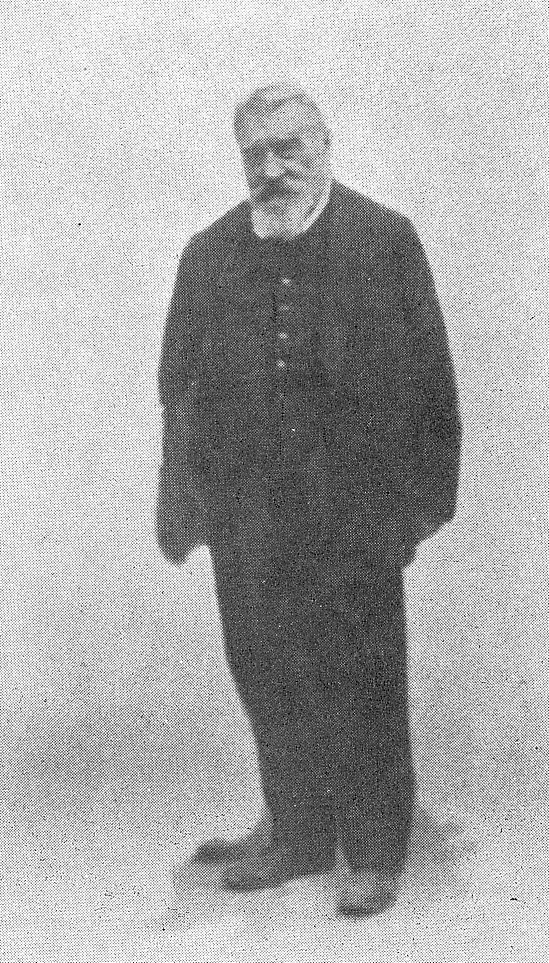
\includegraphics[width=6cm]{alberani}
    \caption[Anselmo Alberani]{\textbf{Anselmo Alberani}\index[Personaggi]{Alberani Anselmo}, uno dei più ricchi proprietari terrieri di Alfonsine, fu pretore. Era il padre di Alberto\index[Personaggi]{Alberani Alberto}, che fu Sindaco di Alfonsine dal 1922 al 1924.\label{fig:alberani}}
    %\vspace{-0.3cm}
\end{figure}